\section{General Root Cause Analysis}
\label{sec:general}

In this section we frame the general problem of locating the root cause
of an arbitrary interdomain path change. For the sake of exposition, we
use an AS as the basic routing element.
%This can be easily generalized
%to finer granularity (\eg PoPs). 
First we make a set of simple observations to 
reason about all possible path changes at a given AS and their implications for root cause analysis. These lead to a a recursive algorithm for isolating the root cause (\S\ref{subsec:rules}).  
%First we develop a simple, yet generic, set of rules for reasoning about a path change and
%present a recursive algorithm for isolating the root cause when
%the complete set of paths toward a prefix is known.
%Because we generally have only an incomplete view of those paths, 
Then we provide a proof as to what is the upper bound on
the set of ASes that our recursive algorithm traverses for root cause
analysis~(\S\ref{subsec:canopy}).
We observe that the number of paths to monitor to obtain this subgraph can
be large for arbitrary path changes. To address this, we use commonly
accepted assumptions about routing decisions to further restrict the set
of monitored paths (\S\ref{subsec:bound}). 

% We show that although the origin of the path change can lie in a
% relatively remote part of the Internet, it still lies within a
% relatively limited sphere of influence starting with the ASes on the
% old and new paths.  

\subsection{Root Cause Analysis Algorithm}
\label{subsec:rules}

We now consider locating the root cause of a change observed on the
path from an AS $v$ towards an AS $s$ that originates a prefix.  In the
following  discussion we isolate the root cause at the granularity of
ASes, but our approach makes few assumptions about routing and can
equally apply to other groupings such as
quasi-routers~\cite{muhlbauer:quasi-router} or PoPs as long as information at these
finer granularities is available.
For simplicity, we assume that at any time there is only one routing event causing a
path change to a particular prefix, and that we have complete and accurate path information.
We revisit these assumptions in \S\ref{sec:design}. We also make the
reasonable assumptions that (i) an AS $v$ changes paths either due to
modifications in its route preference or due to a change in one of its
neighbor's paths or export policies; and that (ii) if $v$ did not change
its next hop to $s$ nor its export policy, it is not responsible for the
route change.  

Below we enumerate all possible observations of path changes at an AS
$v$ and what inference we can make from each observation for root cause
analysis. Let $O(v)$ and $N(v)$ denote the old and the new paths AS
$v$ used before and after the event, respectively.\footnote{Even though the
text focuses on the sequence of ASes in a path, comparison of paths
includes other relevant data such as BGP communities and multi-exit
discriminators when available.}

\nparagraph{\emph{Local change}.}  If AS $v$ changed its next
hop toward $s$, \ie $O(v) = [x, \ldots, s]$ and $N(v) = [y, \ldots, s]$ such that $x \neq y$,
but both next hops did not change paths, \ie $O(x) = N(x)$ and $O(y) =
N(y)$, then the root cause is in $\{v, x, y\}$.  Either $v$ changed its
route preference or either $x$ or $y$ changed their export policy.
If there is no working path before or after a change,
either $x$ or $y$ is null. Note also that if there was no change at $v$, 
\ie $O(v) = N(v) = [x, \ldots, s]$, then downstream ASes $\{x,
\ldots, s\}$ are not the root cause of the event.  AS $v$ can still be
the root cause if it changed its export policy (\ie started or stopped
announcing the route upstream). 

\nparagraph{\emph{Neighbor path change}.} If AS $v$ changed
its next hop toward $s$, \ie $O(v) = [x, \ldots, s]$ and $N(v) = [y,
\ldots, s]$, and one of the neighbors changed paths, \ie $O(x) \ne
N(x)$ or $O(y) \ne N(y)$, then the change at $v$ was induced by the
change in its next hop neighbor and $v$ is not the root
cause. 

\nparagraph{\emph{Downstream change}.}  If the old and new
paths at an AS $v$ share the first hop but downstream hops are
different, \ie $O(v) = [x, \ldots,$ $m, \ldots, s]$ and $N(v) = [x,
\ldots, n, \ldots, s]$, then $v$ is not the root cause of the event.

% \ekb{this could use an argument that it is complete. Either the path
% is the same or it changed. If it changed, either the next hop changed
% or the only change is further downstream. If the next hop changed,
% either the old/new next hops' paths changed or they didn't. We could
% lead in with a discussion of what types of changes could occur, then
% discuss the rules, perhaps.}

\vspace{0.4em}The observations above can be combined to build a generic
root cause identification algorithm as shown in
\algstr~\ref{algo:rules}.  The algorithm starts from an AS $v$ where a
change was observed.  If $v$ uses the same next hop AS toward $s$ before
and after the change, $v$ is not the root cause and we continue our
search downstream (\downstreamC). If $v$ uses different next
hop ASes and one of them changed paths, then we search downstream from the
next hop that changed paths (\neighborC). If both next
hops of an AS $v$ change paths, the changes are due to the same (unique)
root cause and \algstr~\ref{algo:rules} finds the root cause regardless of
the next hop chosen in the recursive call.  If $v$ uses different next
hop ASes before and after the change and the next hops did not change
paths, then we have found the root cause (\localC).

% \begin{pseudocode}[t]
% \textbf{Precondition:} A path change observed on the path from $v$
% to $s$.  Let $O(v) = [v, x, \ldots, s]$ and
% $N(v) = [v, y, \ldots, s]$.\\
% \textbf{RootCause\new{Localization}(v, s):}\\
% %
% {\scriptsize 1}\hspace*{1em}\textbf{if} $x = y$:
% \hfill\emph{// Observation 4 applies}\\
% {\scriptsize 2}\hspace*{2em}\textbf{return} RootCause\new{Localization}$(x, s)$\\
% %
% {\scriptsize 3}\hspace*{1em}\textbf{if} $O(x) = N(x)$ and $O(y) = N(y)$:
% \hfill\emph{// Obs. 2 applies}\\
% {\scriptsize 4}\hspace*{2em}\textbf{return} $\{v, x, y\}$\\
% %
% {\scriptsize 5}\hspace*{1em}\textbf{if} $O(x) \ne N(x)$:
% \hfill\emph{// Obs. 3 applies}\\
% {\scriptsize 7}\hspace*{2em}\textbf{return} RootCause\new{Localization}$(x, s)$\\
% %
% {\scriptsize 8}\hspace*{1em}\textbf{if} $O(y) \ne N(y)$:
% \hfill\emph{// Obs. 3 applies}\\
% {\scriptsize 9}\hspace*{2em}\textbf{return} RootCause\new{Localization}$(y, s)$
% \caption{Recursive algorithm for general root cause analysis using
% observations 1--4.}
% \label{algo:rules}
% \end{pseudocode}


\begin{pseudocode}[t]
\textbf{Precondition:} A path change observed on the path from $v$
to $s$.  Let $O(v) = [v, x, \ldots, s]$ and
$N(v) = [v, y, \ldots, s]$.\\
\textbf{RootCause(v, s):}\\
%
{\scriptsize 1}\hspace*{1em}\textbf{if} $x = y$:
\hfill\emph{// downstream change}\\
{\scriptsize 2}\hspace*{2em}\textbf{return} RootCause$(x, s)$\\
%
{\scriptsize 3}\hspace*{1em}\textbf{if} $O(x) \ne N(x)$:
\hfill\emph{// neighbor path change}\\
{\scriptsize 4}\hspace*{2em}\textbf{return} RootCause$(x, s)$\\
%
{\scriptsize 5}\hspace*{1em}\textbf{if} $O(y) \ne N(y)$:
\hfill\emph{// neighbor path change}\\
{\scriptsize 6}\hspace*{2em}\textbf{return} RootCause$(y, s)$

{\scriptsize 7}\hspace*{1em}\textbf{return} $\{v, x, y\}$
\hfill\emph{// local change}%
%
\caption{Recursive algorithm for general root cause analysis.}
\label{algo:rules}
\end{pseudocode}

We can simplify inference from a \localC{} if we assume that ASes do not
change their export policy, \ie if an AS is (is not) exporting a
particular path to a particular neighbor, it will not stop (start)
exporting to that neighbor unless it changes paths.  Under this
assumption,  ASes $x$ and $y$ cannot be the root cause in a \localC{}.
Simply put, if $O(x) = N(x)$, $x$ is not the root cause. As a result,
line 7 of \algstr~\ref{algo:rules} would return only $\{v\}$ as the root
cause.

% As an example, consider the path change in \fig~\ref{fig:induced1}.  The
% algorithm starts from AS $v$ where $O(v) = [x, b, a, s]$ and $N(v) = [y,
% e, s]$, and $O(y) \ne N(y)$.  We apply Rule~4 and search for the root
% cause downstream $y$ (lines 6--9).  At $y$ we have $O(y) = [z, d, c,
% s]$, $N(y) = [e, s]$, and $O(z) \ne N(z)$.  Again, we we call the
% algorithm recursively to search for the root cause downstream $z$.  At
% $z$ we have $O(z) = [d, c, s]$, $N(z) = \emptyset$, and both neighbors
% ($d$ and $\emptyset$) have the same paths before and after the failure.
% The algorithm applies Rule~2 and returns $\{z, d, \emptyset\}$ as the
% root cause.  Under the assumption that export policies are fixed, we
% would get $\{z\}$ as the root cause.

As an example, \tab~\ref{tab:alg1.fig1} shows the steps taken by
\algstr~\ref{algo:rules} when applied to the path change in
\fig~\ref{fig:induced1}. The algorithm starts at $v$, observes a
\neighborC{} since the old and new first hops are different, and calls
itself recursively to search the root cause downstream from $y$.  At
$y$, the algorithm observes another \neighborC{} and
searches the root cause downstream from $z$. At $z$, the algorithm
observes a \localC{} and identifies $\{z, d, \emptyset\}$ as the
root cause as both neighbors ($d$ and $\emptyset$) did not change paths
($\emptyset$ is $z$'s neighbor since $z$ has no new path due to the
failed link $z-d$). Under the assumption that export policies are fixed,
we would get $\{z\}$ as the root cause instead.

\begin{table}[t]
\begin{center}
\begin{tabular}{ccccc}
Recursion & Target & \multirow{2}{*}{$O(\cdot)$} &
\multirow{2}{*}{$N(\cdot)$} &\multirow{2}{*}{Observation} \\
Depth & AS & & & \\
1 & $v$ & $[x, b, a, s]$ & $[y, e, s]$ & \emph{neighbor path change} \\
2 & $y$ & $[z, d, c, s]$ & $[e, s]$ & \emph{neighbor path change} \\
3 & $z$ & $[d, c, s]$ & $\emptyset$ & \emph{local change} \\
\end{tabular}
\caption{An example of \algstr~\ref{algo:rules} applied to the path change
shown in \fig~\ref{fig:induced1}.}
\label{tab:alg1.fig1}
\end{center}
\end{table}

\subsection{General Candidate and Monitored Sets}
\label{subsec:canopy}

We now consider the set of ASes that \algstr~\ref{algo:rules} could
traverse for an arbitrary path change observed at $v$, 
which yields the full set of path information that the algorithm could require 
to identify the root cause.

We define the \emph{general candidate set} of an AS $v$, denoted
$\mathcal{C}(v)$, as the set of ASes \algstr~\ref{algo:rules} may identify
as the root cause of a path change observed at $v$. For a given
path change for prefix $p$ observed at AS $v$, $\mathcal{C}(v)$ is a set
containing $v$ itself and the ASes in the general candidate sets of its
old and new 
downstream neighbors.  Let $O_{\mathrm{n}}(v)$ and $N_{\mathrm{n}}(v)$
denote the downstream \textbf{n}eighbors AS $v$ chose toward $p$ before and after
the change, respectively. Then $\mathcal{C}(v) = v \cup
\mathcal{C}(O_{\mathrm{n}}(v)) \cup \mathcal{C}(N_{\mathrm{n}}(v))$.
 
As an example, in \fig~\ref{fig:induced1}, $O_{\mathrm{n}}(v) = x$,
$N_{\mathrm{n}}(v) = y$, and the general candidate set of $v$ contains
the ASes in $v$'s old and new paths ($v, x, b, a, y, e, s$) as well as
the ASes in $y$'s old path ($z, d, c$). If $z$ had a new path, its ASes
would also be in $\mathcal{C}(v)$.  ASes like $m$ and $n$ that are not
involved in the change are not in $v$'s general candidate set.  Now we can
prove the following result. 

\begin{theorem}
If there is only one routing event in the network, the root cause of a path
change at an AS $v$ lies in $\mathcal{C}(v)$.
\label{thm:correctness}
%\vspace{-1.5em}
\end{theorem}

\begin{proof}  The claim is trivially true if the root cause is $v$. If
there is another AS $x$ in $O(v)$ or $N(v)$ that changed paths, the
change at $v$ was induced by the downstream change at $x$ (\neighborC{}
or \downstreamC{}).  Such an AS $x$ is in $\mathcal{C}(v)$.  Similarly,
if there is another AS $y$ in $O(x)$ or $N(x)$ that changed paths, the
change at $x$ was induced by the change at $y$.  Such an AS $y$ is in
$\mathcal{C}(x) \subset \mathcal{C}(v)$.  We can follow this process
recursively until we find the AS $c \in \mathcal{C}(v)$ that is the AS
closest to the source that changed paths (\ie there is no AS downstream
$c$ that changed paths).  Without loss of generality, we need to prove
that the root cause of the change at $c$ is in $\mathcal{C}(v)$. An AS
not in $O(c) \cup N(c)$ cannot be the cause of the change at $c$ because
it cannot change the relative preference between the (unchanged) paths
$c$ receives from its downstream neighbors $O_\mathrm{n}(c)$ and
$N_\mathrm{n}(c)$.  Thus, either $c$ changed its route preference and is
the root cause, or one of its downstream neighbors changed their export
policy and are the root cause (\localC{}).  This
completes the proof.\hfill\qed \end{proof}

\algstr~\ref{algo:rules} is guaranteed to identify the root cause of path
changes. However, it requires path information from a potentially large set of
ASes in the network.  Identifying the root cause of a change at an AS
$v$ requires information about the old path used by an AS $x$ in the new
path chosen by~$v$, \ie we need to know $O(x)$, where $x \in N(v)$.
Because we cannot know the ASes in $N(v)$ until after the path change,
we need to track the old paths from all ASes in all possible paths $v$
can change into.  For example, in \fig~\ref{fig:induced1}, we need to
monitor paths from $x$, $y$, and $m$, as we do not know {\em a priori} what neighbor
$v$ will choose after a change.  Given the recursive calls in
\algstr~\ref{algo:rules}, the set of ASes we need to track paths from may
grow exponentially with the path length, subject to the upper bound of
the size of the AS graph.

Formally, we define the \emph{general monitored set} of an AS $v$,
denoted $M(v)$, as the set of ASes whose old paths we need to track to
run \algstr~\ref{algo:rules} on path changes observed at AS $v$.  Let
$L(v)$ denote the set of neighbor ASes $v$ can use to reach an AS $s$.
The set $M(v)$ includes the neighbors $v$ can use to reach $s$ and all
ASes in the general monitored sets of each of $v$'s neighbors.  This
gives $M(v) = L(v) \cup \{M(x) \mid x \in L(v)\}$.  While the general candidate set, 
$\mathcal{C}(v)$, is specific to a given change, $M(v)$ is not and covers
all possible changes. Note that $\mathcal{C}(v) \subset M(v)$, as $\mathcal{C}(v)$ includes the general candidate set of
only the neighbors $v$ chose before and after the path change. For
example, in \fig~\ref{fig:induced1}, $\mathcal{C}(v)$ includes
$\mathcal{C}(x)$ and $\mathcal{C}(y)$, while
$M(v)$ includes $M(x)$, $M(y)$, and $M(m)$.

% For example, if all paths from AS $v$ to a destination AS $d$ have
% five ASes, each AS has three next hop ASes, and there is no overlap,
% then we need to monitor paths from $243 = 3^5$ ASes.

\begin{comment} % {{{
\subsection{General Root Cause Analysis with Perfect Information (old
version, candidate for removal, theoretic content above needs double
checking)}

\tbd{Secs. 3.1 and 3.2 has a lot of overlap with the content in this
section.  I moved the two main points here to Sec. 3.2: (1) the canopy
set contains the root cause and (2) we have to monitor a lot of paths to
make sure we have information about all ASes in the canopy set.  I think
we may remove this section after we integrate other important points in
3.1 and 3.2.}

An algorithm for general root cause analysis must account for the fact that 
routing changes can take place due to decisions made at a relatively distant AS. 
These decisions can be the result of an event internal to a given AS or at the boundary
between two ASes. Consider, for example, \fig~\ref{fig:recur}, where AS $D$ announces prefix $p$
to the Internet, observed at a vantage point located in AS $V$.
Initial paths are represented by dashed lines and data is forwarded
in the direction of the arrows. Paths after the routing event are represented by
solid lines. Suppose that a failure occurs on the path from $C$ to $D$, resulting in
$C$ withdrawing that path from $B$. This causes $B$ to switch to a path through $E$. As it happens,
$B$'s peer $A$ prefers this new path over its old path through $G$, causing $A$ to switch 
its paths as well. Finally, $V$ prefers the path through $F$ to this new path advertised by $A$. 
Hence we observe a new path through $A$ and $G$ at $V$ toward prefix $p$. 
\tbd{maybe change the example to a real case of induced path change we
identified; for example, an induced change caused by a localpref in an
AS may be more intuitive}

In this case, a routing change originally impacting $C$ has caused three other ASes to change their paths 
in a cascading fashion. In each case, the AS making the decision observes a change on its most preferred path
at that time: either the most preferred path is withdrawn or becomes available, causing the AS to switch to
its second favorite path in the former case or switch back to its favorite path in the latter case. This cascading pattern suggests that although the original link failure lies faraway from the ASes involved in the path change observed at $V$, it is not completely arbitrary. In fact, it lies within the canopy of ASes created by considering the top two paths preferred by each AS encountered as we move from the vantage point AS to the destination AS. We formalize this observation in theorem. Assume that i) a path change was caused by a single routing event, ii) all paths are stable (convergence has taken place), iii) an AS exports the same path to all its neighbors for a given destination \ekb{should also allow it to export no paths to some neighbor. This is also confusig given the granularity challenge above.}, and iv) an AS selects a path to a destination based on a total ordering over all available paths. We observe that a path change observed at a vantage point involves a sequence of ASes whose next-hops are different after the routing event: either there's another next-hop AS or there is none (due to link failure/restoration). We call these \emph{divergent ASes}. For example, the set of divergent ASes in \fig~\ref{fig:recur} is ${V, A, B, C}$. The \emph{root-cause AS} is defined as the first divergent AS in this sequence \ekb{haven't defined the ordering}, e.g., $C$. Notice that in case of an \emph{induced} path change, as depicted in \fig~\ref{fig:recur}, the root-cause AS does't lie on the old or new paths observed at the vantage point.

We now prove a bound on the number of ASes needed to monitor to find the root-cause AS of an arbitrary interdomain path change. The \emph{canopy set} is defined as:

\begin{definition}
%
For a given path change for prefix $p$ observed at AS $a$, the
\emph{canopy set} of $a$, $\mathcal{C}(a)$, is a set containing $a$
itself and the ASes in the canopy sets of the downstream neighbors $a$
chose toward $p$ before and after the change.  Let
$N_\mathrm{before}(a)$ and $N_\mathrm{after}(a)$ denote the downstream
neighbors $a$ chose to route packets to $p$ before and after the change,
respectively; then $\mathcal{C}(a) = a \cup
\mathcal{C}(N_\mathrm{before}(a)) \cup
\mathcal{C}(N_\mathrm{after}(a))$.
%
\end{definition}
 
 As an example, for the path change shown in \fig~\ref{fig:recur}, $V$'s canopy set \textbf{C} includes all ASes
 shown. In addition to all ASes appearing in $V$'s old and new paths ($V$, $A$, $G$, $D$ and $F$), ASes on $A$'s 
 new path ($B$ and $E$) and $B$'s old path ($C$) are included in the canopy set.

\begin{theorem}
For a path change observed at vantage point $V$ toward destination $D$, all divergent ASes appear in
$V$'s canopy set.
\label{thm} 
\end{theorem}

\begin{proof}
The proof is by induction. For the base case, there is obviously at least one divergent AS lying on either the
old or new path from $V$, or otherwise there would be no path change. Since this AS appears on either the
old or new path from $V$, it is included in the canopy set \textbf{C}. 
For the general case, suppose the divergent AS $X$ lies in \textbf{C}. Since $X$ is divergent, there are 
three cases: i) it has two different paths either side of the routing event with with different first-hops, $Y$ and $Z$,
ii) it only has one path through $Y$ before the routing event, iii)  it only has one path through $Z$ after
the routing event. Dealing with first case (the other two are similar) and without loss of generality assume $Y$
is the next divergent AS. Since $Y$ lies on either of the two most preferred paths $p_X$ or $q_X$, Y lies in the
canopy set \textbf{C} of $V$. \qed
\end{proof}

Theorem~\ref{thm} leads us to conclude:

\begin{corollary}
For a path change observed at vantage point $V$ toward destination $D$, the root-cause AS appears in
$V$'s canopy set.
\label{cor} 
\end{corollary}

\begin{proof}
Since the root-cause AS is the first divergent AS, by Theorem~\ref{thm} it resides in \textbf{C}. \qed  
\end{proof}

This suggests a general recursive algorithm to pinpoint the root-cause
a sketch of which is presented in \fig~\ref{fig:gen-algo}. 
We assume that a path change from the old path
$O(V)$ to the new path $N(V)$ is observed at vantage point $V$. 
The algorithm starts at $V$ and each level of recursion
begins at an AS where the old and new paths diverge. For example, 
in \fig~\ref{fig:recur} $V$ is the vantage point at level 1 since 
it is where the first path change is observed, $A$ is the vantage point for 
level 2, and so on. Notice that the recursion halts when it reaches 
the origin of the prefix, i.e., $D$.

\begin{pseudocode}
%\framebox[\columnwidth][l]{
%\parbox{\columnwidth}{
\textbf{RootCause} at AS $V$ \\
\textbf{Given:} $O(V)$ and $N(V)$ toward destination AS $D$ \\
\hrule
\textbf{if} $O(V)$ is the same as $N(V)$: \\ %or current recursion depth is $D$ \\
\hspace*{0.2in} \textbf{return} $\mathcal{\emptyset}$ \\
\textbf{for each} AS $A$ in $O(V)$ in order of propagation from $D$: \\
   \hspace*{0.2in} \textbf{if} $A$ has already been visited \textbf{then continue} \\
   \hspace*{0.2in} \textbf{R}$(A) \leftarrow$ \textbf{RootCause} at AS $A$ \\
   \hspace*{0.2in} \textbf{if} \textbf{R}$(A) \ne
\mathcal{\emptyset}$ \textbf{then} \textbf{return} \textbf{R}$(A)$:  \\
\textbf{for each} AS $A$ in $N(V)$ in order of propagation from $D$ \\
   \hspace*{0.2in} \textbf{if} $A$ has already been visited \textbf{then continue} \\
   \hspace*{0.2in} \textbf{R}$(A) \leftarrow$ \textbf{RootCause} at AS $A$ \\
   \hspace*{0.2in} \textbf{if} \textbf{R}$(A) \ne
\mathcal{\emptyset}$ \textbf{then} \textbf{return} \textbf{R}$(A)$  \\
\textbf{return} $V$

\caption{General recursion-based algorithm for discovering root-cause}
\label{fig:gen-algo}
\end{pseudocode}

\end{comment} % }}}

\subsection{Bounding Candidate and Monitored Sets}
\label{subsec:bound}

To address the challenge of monitoring a prohibitively large set of
ASes, we provide a bound on the general candidate set $\mathcal{C}(v)$.
We then use this bound to reduce the set of ASes we need to monitor to
perform root cause analysis.

% We bound the set of candidate ASes using the assumption that ASes use
% three criteria for path selection: (i) economic utility (referred to
% as EU), where ASes set route preferences based on business
% relationships, \eg ASes usually prefer paths through customers over
% paths through peers over paths through providers; (ii) network utility
% (NU) which optimizes for intra-domain traffic, \eg early exit; and
% (iii) social utility (SU) wherein ASes prefer shorter AS paths.  We
% assume EU trumps NU which in turn trumps SU.

Our bound on the candidate set is derived from the simple and widely
used Gao-Rexford routing model~\cite{gao}; \ie we assume each AS
has a total ordering over the preferences for all available paths toward a
prefix. For example, an AS typically prefers a path learned from a
customer over another learned from a peer or provider, and a path
learned from a peer over another learned from a provider.

We also assume an AS considers its LocalPref (which can encode policies
such as business relationships and/or traffic engineering) for each
path before AS path length when selecting among paths
announced by multiple neighbors toward the same prefix.  This assumption
is reasonable as it is used in the BGP route selection process.
The shorter path is picked only if two or more paths have the same
LocalPref (\eg both are customer paths).

We further assume that assigning LocalPref values
only on neighboring ASes. In other words, path preference at an AS 
does not depend on which specific ASes are in the path, except for the next hop ASes only, 
a property that holds empirically the vast majority of the time~\cite{gill:nanog}.

\begin{figure}[t]
\centering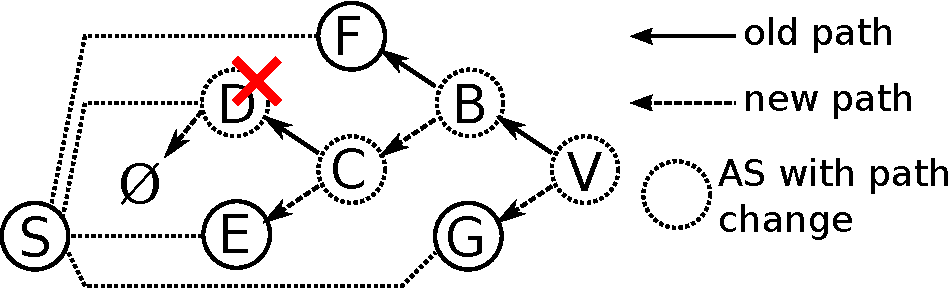
\includegraphics[width=\columnwidth]{figs/induced3b.pdf}
\vspace{-5mm}
%
\caption{General topology subgraph demonstrating a three-level induced
path change starting at $\boldsymbol{c}$ and propagating up to
$\boldsymbol{v}$ (impossible under the simplified routing model).  The
ASes shown can be anywhere in the path.}
%
\label{fig:induced3}
\end{figure}

Based on this routing model we
identify the ASes from the general candidate set most likely to have
caused a path change. We overload our notation for the old and new paths used by an AS $v$,
$O(v)$ and $N(v)$, as follows. $N(O(v))$ is the set of ASes that appear
on the new paths originating from the ASes in $O(v)$, and $O(N(v))$ is
the set of ASes that appear on the old paths originating from ASes in
$N(v)$.  For example, in \fig~\ref{fig:induced3}, $O(v) = [b, f, \ldots,
s]$ and $N(O(v)) = O(v) \cup N(b) \cup N(f) \cup \cdots \cup N(s) = \{b,
f, c, e, \ldots, s\}$.

\begin{theorem} Under the simplified routing model, the root cause of a
path change observed at an AS $a$ is contained in the \emph{bounded candidate
set} $\mathcal{B}(v) = N(O(v)) \cup O(N(v))$.
\end{theorem}

\begin{proof}

We first show that
the root cause AS \emph{may} appear in $\mathcal{B}(v)$. It is obvious
that the root cause may lie on either the old or the new path, \ie ASes
like $g$ and $b$.  ASes in the set $N(O(v))$, like $c$, can be the root
cause as well.  Using \fig~\ref{fig:induced3} as an example, suppose a failed link $c$--$b$ comes back
up and $c$ starts announcing a path to $b$. AS $b$ may start routing
through $c$ if it prefers paths from $c$ over paths from $f$.  AS $v$
may then change its route from $b$ to $g$ if the new path through $[b,
c, \ldots, s]$ is longer.  The case of $O(N(v))$ is similar.

Now we show that ASes in the set $\mathcal{C}(v) - \mathcal{B}(v)$
cannot be the root cause.  These include ASes like $d$, which lies in
$O(N(O(v)))$.  Proceeding by contradiction, assume that the path change
shown in \fig~\ref{fig:induced3} happens and that the root cause is $d$,
causing $c$ to switch to a different path through $e$ and causing $b$ to
switch to $c$'s new path.  This implies that $b$'s criterion for path
selection between $f$ and $c$ is path length.  If $b$ had a policy
favorable to $c$ (\eg a higher LocalPref for $c$) then it would have
picked the path through $c$ in the first place. If $b$ had a policy
favorable to $f$ it would not change paths. Shortest path routing at
$b$ implies that $[b, c, e, \ldots, s] \leq [b, f, \ldots{}, s] \leq [b,
c, d, \dots{}, s]$, where the `$\leq$' operator compares path lengths.
This is because $b$ prefers the path through $f$ before the routing
event and the path through $c$--$e$ after.  Now, if $v$ switches to the
new path through $g$, then it implies that $v$ is using shortest path
routing to choose between $b$ and $g$.  As $v$ prefers the path through
$b$--$f$ over the path through $g$ before the routing event and the path
through $g$ over the path through $b$--$c$ after, we have that $[v, b,
f, \ldots{}, s] \leq [v, g, \ldots{}, s] \leq [v, b, c, e, \ldots, s]$.
Looking at the paths from $v$ we have that $[b, f, \ldots{}, s] \leq [b,
c, e, \ldots{}, s]$. This contradicts the earlier result from $b$ that
$[b, c, e, \ldots{}, s] \leq [b, f, \ldots{}, s]$.  Hence, $d$ or any
other AS in $O(N(O(v)))$ cannot be the root cause.  The argument is
similar for $N(O(N(v)))$.  {\color{white}wrapwrap}\hfill\qed \end{proof}

Observe that $\mathcal{B}(v) = N(O(v)) \cup O(N(v))$ is contained in
$v$'s general candidate set $\mathcal{C}(v)$.  Hence, if the root cause
lies in $\mathcal{B}(v)$, it also lies in $\mathcal{C}(v)$, as per
Theorem~\ref{thm:correctness}.
Note also that if our assumptions and routing model are wrong, the root cause
of a path change at $v$ can lie outside $\mathcal{B}(v)$.  However, we
\emph{can} still detect violations of the assumptions checking that the
root cause is outside $\mathcal{B}(v)$.

\begin{comment} % {{{
Even if we limit our search for the root cause in the bounded candidate
set $\mathcal{B}(v) = N(O(v)) \cup O(N(v))$, the $O(N(v))$ term implies
we need to track the old paths from all ASes that may appear in any new
path $v$ can choose.  This makes the set of ASes whose old paths we need
to track the same as the general monitored set $M(v)$.  To bound the
monitored set, we only track the old paths from ASes in the most
preferred paths $v$ can change to.  

We define the \emph{bounded monitored set}, denoted $T(v)$, as the set
of ASes in all paths that $v$ prefers over $O(v)$ plus the ASes from the
next preferred path from each AS in $O(v)$.  AS $v$ may change away from
$O(v)$ if a more preferred path becomes available.  In this case we have
complete information to run root cause analysis as the monitored set
$T(v)$ includes all ASes in paths that are more preferred than $O(v)$.
Conversely, AS $v$ may change away from $O(v)$ to a less preferred path
if $O(v)$ becomes unavailable.  In these cases, we only miss information
when an AS $x \in O(v)$ changes to a path that is not its next preferred
path (which may happen, \eg when the network lacks redundancy and an
event impacts both of an AS's current and next preferred path).  If path
preference information is unavailable for an AS $v$, we take a
conservative approach and add the best path from each of $v$'s
downstream neighbors to $T(v)$.
\end{comment} % }}}

% We define the \emph{bounded monitored set}, denoted $T(v)$, as the set
% of ASes in all paths from $\boldsymbol{p}_0$ to $\boldsymbol{p}_{j}$,
% where $j > i$ is the index of the most preferred path after $i$ such
% that $\boldsymbol{p}_i$ and $\boldsymbol{p}_j$ are disjoint.  That is,
% $T(v) = \{x \mid x \in \boldsymbol{p}_k, 0 \le k \le j\}$.  

Even if we limit our search for the root cause in the bounded candidate
set $\mathcal{B}(v) = N(O(v)) \cup O(N(v))$, the $O(N(v))$ term implies
we need to track the old paths from all ASes that may appear in any new
path $v$ can choose.  This makes the set of ASes whose old paths we need
to track the same as the general monitored set $M(v)$.

To bound the monitored set, we only track the old paths from ASes in the
most preferred paths $v$ can change to.  AS $v$ may change away from
$O(v)$ if a more preferred path becomes available.  To cover this case,
we monitor old paths from all ASes in paths that are more preferred than
$O(v)$.  Conversely, AS $v$ may change away from $O(v)$ to a less
preferred path if $O(v)$ becomes unavailable. Monitoring old paths from
all ASes in paths that are less preferred than $O(v)$ can be costly and
wasteful because $v$ should use preferred paths most of the time and the
less preferred a path, the less likely it will be used.  Instead, we
monitor old paths from all ASes in the next less preferred paths from
each AS $x$ in $O(v)$.  This approach only misses information when an AS
$x \in O(v)$ changes to a path that is not its next less preferred path
(which may happen, \eg when the network lacks redundancy and an event
impacts both of an AS's current and next preferred path).

%\ekb{This does make me wonder a bit if we should do something (in the future)
%in terms of monitoring paths that don't overlap, to guard against all changes.}

We define the \emph{bounded monitored set}, denoted $T(v)$, as the
set of ASes in all paths that $v$ prefers over $O(v)$ plus the ASes from
the next less preferred path from each AS in $O(v)$.  If path preference
information is unavailable for an AS $v$, we take a conservative
approach and add the most preferred path from each of $v$'s downstream neighbors
to $T(v)$.  We have that $T(v) \subset M(v)$.  We also note that while
$\mathcal{B}(v)$ is specific to a given change, $T(v)$ is not and covers
most possible changes.

Tracking paths from ASes in the most preferred paths reduces the
monitored set when identifying the root cause in the bounded candidate
set $\mathcal{B}(v)$ because we need to know only $O(N(v))$.  
%\drc{I think this paragraph is here to make it clear that there is value in 
%the bound, but I didn't find myself asking the question of whether it would 
%be useful for C(a). Do we really need this?}
The
heuristic would not be as effective at reducing the monitored set if we were
identifying the root cause using the general candidate set
$\mathcal{C}(v)$.  The reason is that we would need to monitor ASes in
the most preferred paths for any AS that can show up in new paths,
recursively.  For example, we would need to track ASes that can show up
in the most preferred paths of all ASes in $N(O(v))$ to know
$O(N(O(v)))$.

\begin{comment}
\subsection{Monitoring the ASes in the Candidate Set}
\label{subsec:monitor}
\drc{This should move to section 4.3.}

Now that we have a bound on the set of ASes we need to monitor to
perform root cause analysis, a measurement framework needs to be put in
place that would incrementally identify the ASes in this set and to
track the paths they use. 

% This may be achieved through a combination of passive and active
% measurements from a globally distributed set of vantage points, such
% as RouteViews~\cite{ripe-ris,routeviews} for BGP paths or the
% Planetlab testbed~\cite{planetlab} for traceroutes. 

\noindent\textbf{Passive Monitoring of Paths to Prefixes.} One way to
identify the ASes in the monitored set $T(v)$ is to continuously monitor
public BGP feeds~\cite{ripe, routeviews}.  Each BGP update contains one
path an AS $x$ can use to reach another AS.  Monitoring changes for a
prolonged period of time allows us to discover a set of paths an AS may
use to reach a prefix $x$ and build the set of ASes we need to monitor
to perform root cause analysis.  Although a passive approach reveals
actual paths used in the Internet and is minimally invasive, waiting for
actual path changes to take place is likely going to be slow for the
purposes of identifying the ASes needed to be monitored.  \tbd{Can't we
just take a longer history to mitigate the slowness?}  Another problem
is that not all paths appear in BGP feeds because ASes only propagate
their best path, export filters, and prefix aggregation. \drc{I think these last 
two sentences are backwards. The lack of complete information means 
that these feeds need to be supplemented with active measurements. That's 
where the point about identifying ASes to be monitored comes in.}

\noindent\textbf{Active Monitoring of Paths to Prefixes.} We can
complement passive BGP data with active traceroute measurements to
periodically collect paths from a set of distributed vantage points to a
set of destination ASes.  One advantage is that traceroute gives us path
information at the granularity of router interfaces, while BGP feeds
give us information at the granularity of ASes.  Unfortunately,
traceroutes add load on the network and the process of converting
traceroute paths to AS paths is prone to
errors~\cite{ono-sidewalk-ends}.

% Second, we need path measurements from each AS at fine enough
% granularity such that the path is available before and after a routing
% change occurs.  We also want to collect all necessary information and
% identify the root cause before the next routing event happens.  Given
% the large set we need to monitor paths from, it may be impossible to
% collect measurements frequently enough.

\begin{figure}[!htbp]
\centering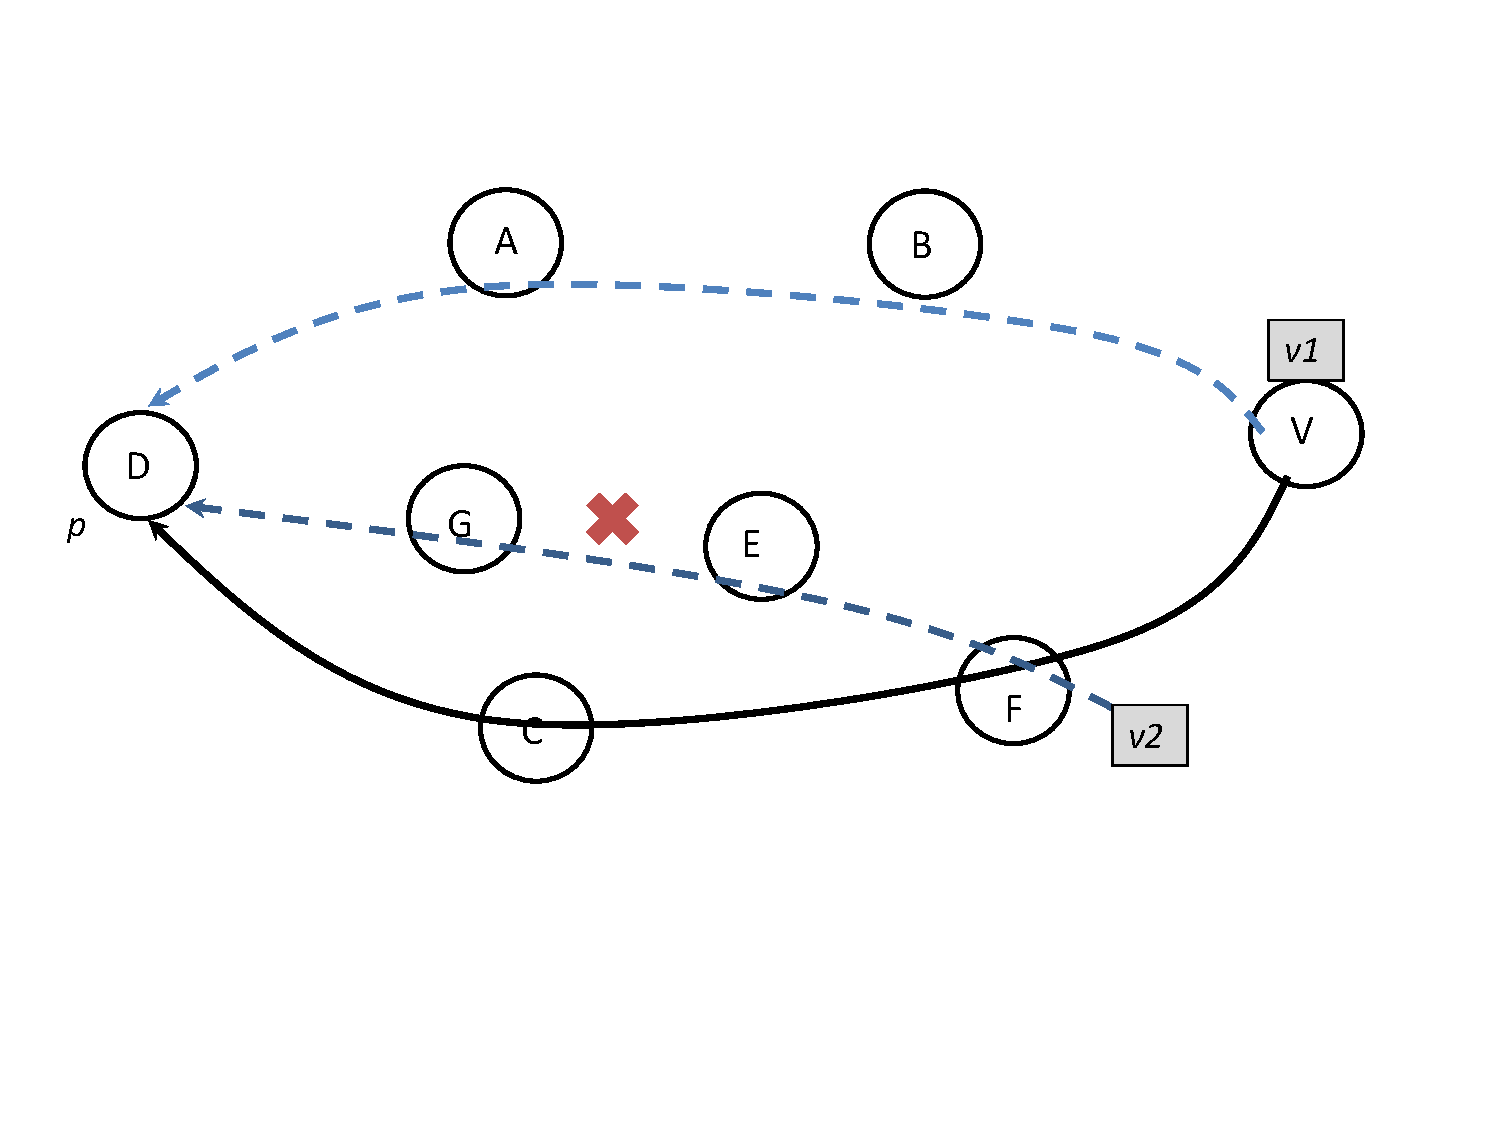
\includegraphics[width=\columnwidth]{figs/computeset.pdf}
\caption{Identifying ASes in the root cause candidate set. When a path change
is observed at vanatge point \emph{v1} (dashed to solid line), 
current and historical paths are queried from other vantage 
points such as \emph{v2} that might have passed through ASes in the old
and new paths. For example, the path from \emph{v2} passes through $F$, an AS
on the new path from $V$ to $D$, allowing us to find out ASes on the
older path from $F$.}
\label{fig:computeset}
\end{figure}

\noindent\textbf{Path Prediction.} At the other end of the spectrum is
offline prediction of policy-compliant paths that an AS is likely to
select when its current path to the destination becomes unavailable or
when new paths become available.  Due to a general lack of access to an
AS's internal routing tables, obtaining knowledge of hidden paths and
local preferences over those paths is far from straightforward.  Using
path prediction techniques from \emph{iPlane}~\cite{iplane}, one can
obtain a set of paths from an AS $x$ to the destination and try to
monitor all ASes that appear in these paths.  Although promising to be
exhaustive, this approach will likely yield a large number of policy
compliant paths (most of which are unlikely to be ever used) and may
lead to a prohibitively large set of ASes to monitor.  

\noindent\textbf{Revealing Alternative Paths via BGP Announcements.}
\drc{We need to say what we are doing before saying what it does.}
This approach emulates a change in link availability and hence forces a
path change.  It is a middle ground between monitoring of path changes
in the wild and prediction of policy-compliant paths.  If an AS $s$ that
originates a prefix wants to discover alternative paths that another AS
$x$ has to its prefix, it can choose $x$'s next hop (or another
downstream AS), say $O_\mathrm{n}(x)$, and prepend that AS in its
announcement for that prefix.  When $O_\mathrm{n}(x)$ receives the
prepended announcements, it rejects the route due to BGP loop detection.
This, in turn, forces $x$ to use the next best route available toward
$s$.  This technique is commonly referred to as BGP
`poisoning'~\cite{optometry, lorenzo-thesis}.  For example, in
\fig~\ref{fig:induced3} poisoning $c$ emulates a link failure between
$c$ and $b$.  This causes $c$ to withdraw the route to $b$, making $b$
use the route through $d$.  By systematically and cumulatively poisoning
ASes in the paths used by AS $x$ to reach $d$, we can discover paths
from $x$ to $s$.  Also, we can infer local preferences at $x$ by looking
at the order in which $x$ picks paths as we poison ASes.

\end{comment}
